%%% Hlavní soubor. Zde se definují základní parametry a odkazuje se na ostatní části. %%%

%% Verze pro jednostranný tisk:
% Okraje: levý 40mm, pravý 25mm, horní a dolní 25mm
% (ale pozor, LaTeX si sám přidává 1in)
\documentclass[12pt,a4paper]{report}
\setlength\textwidth{145mm}
\setlength\textheight{247mm}
\setlength\oddsidemargin{15mm}
\setlength\evensidemargin{15mm}
\setlength\topmargin{0mm}
\setlength\headsep{0mm}
\setlength\headheight{0mm}
% \openright zařídí, aby následující text začínal na pravé straně knihy
\let\openright=\clearpage

%% Pokud tiskneme oboustranně:
% \documentclass[12pt,a4paper,twoside,openright]{report}
% \setlength\textwidth{145mm}
% \setlength\textheight{247mm}
% \setlength\oddsidemargin{14.2mm}
% \setlength\evensidemargin{0mm}
% \setlength\topmargin{0mm}
% \setlength\headsep{0mm}
% \setlength\headheight{0mm}
% \let\openright=\cleardoublepage

%% Vytváříme PDF/A-2u
\usepackage[a-2u]{pdfx}

%% Přepneme na českou sazbu a fonty Latin Modern
\usepackage[czech]{babel}
\usepackage{lmodern}
\usepackage[T1]{fontenc}
\usepackage{textcomp}

%% Použité kódování znaků: obvykle latin2, cp1250 nebo utf8:
\usepackage[utf8]{inputenc}

%%% Další užitečné balíčky (jsou součástí běžných distribucí LaTeXu)
\usepackage{amsmath}        % rozšíření pro sazbu matematiky
\usepackage{amsfonts}       % matematické fonty
\usepackage{amsthm}         % sazba vět, definic apod.
\usepackage{bbding}         % balíček s nejrůznějšími symboly
			    % (čtverečky, hvězdičky, tužtičky, nůžtičky, ...)
\usepackage{bm}             % tučné symboly (příkaz \bm)
\usepackage{graphicx}       % vkládání obrázků
\usepackage{fancyvrb}       % vylepšené prostředí pro strojové písmo
\usepackage{indentfirst}    % zavede odsazení 1. odstavce kapitoly
\usepackage{natbib}         % zajištuje možnost odkazovat na literaturu
			    % stylem AUTOR (ROK), resp. AUTOR [ČÍSLO]
\usepackage[nottoc]{tocbibind} % zajistí přidání seznamu literatury,
                            % obrázků a tabulek do obsahu
\usepackage{icomma}         % inteligetní čárka v matematickém módu
\usepackage{dcolumn}        % lepší zarovnání sloupců v tabulkách
\usepackage{booktabs}       % lepší vodorovné linky v tabulkách
\usepackage{paralist}       % lepší enumerate a itemize
\usepackage{xcolor}         % barevná sazba

%%% Údaje o práci

% Název práce v jazyce práce (přesně podle zadání)
\def\NazevPrace{Název práce}

% Název práce v angličtině
\def\NazevPraceEN{Name of thesis}

% Jméno autora
\def\AutorPrace{Jméno Příjmení}

% Rok odevzdání
\def\RokOdevzdani{ROK}

% Název katedry nebo ústavu, kde byla práce oficiálně zadána
% (dle Organizační struktury MFF UK, případně plný název pracoviště mimo MFF)
\def\Katedra{Název katedry nebo ústavu}
\def\KatedraEN{Name of the department}

% Jedná se o katedru (department) nebo o ústav (institute)?
\def\TypPracoviste{Katedra}
\def\TypPracovisteEN{Department}

% Vedoucí práce: Jméno a příjmení s~tituly
\def\Vedouci{Vedoucí práce}

% Pracoviště vedoucího (opět dle Organizační struktury MFF)
\def\KatedraVedouciho{katedra}
\def\KatedraVedoucihoEN{department}

% Studijní program a obor
\def\StudijniProgram{studijní program}
\def\StudijniObor{studijní obor}

% Nepovinné poděkování (vedoucímu práce, konzultantovi, tomu, kdo
% zapůjčil software, literaturu apod.)
\def\Podekovani{%
Poděkování.
}

% Abstrakt (doporučený rozsah cca 80-200 slov; nejedná se o zadání práce)
\def\Abstrakt{%
Abstrakt.
}
\def\AbstraktEN{%
Abstract.
}

% 3 až 5 klíčových slov (doporučeno), každé uzavřeno ve složených závorkách
\def\KlicovaSlova{%
{klíčová} {slova}
}
\def\KlicovaSlovaEN{%
{key} {words}
}

%% Balíček hyperref, kterým jdou vyrábět klikací odkazy v PDF,
%% ale hlavně ho používáme k uložení metadat do PDF (včetně obsahu).
%% Většinu nastavítek přednastaví balíček pdfx.
\hypersetup{unicode}
\hypersetup{breaklinks=true}

%% Definice různých užitečných maker (viz popis uvnitř souboru)
%%% Tento soubor obsahuje definice různých užitečných maker a prostředí %%%
%%% Další makra připisujte sem, ať nepřekáží v ostatních souborech.     %%%

%%% Drobné úpravy stylu

% Tato makra přesvědčují mírně ošklivým trikem LaTeX, aby hlavičky kapitol
% sázel příčetněji a nevynechával nad nimi spoustu místa. Směle ignorujte.
\makeatletter
\def\@makechapterhead#1{
  {\parindent \z@ \raggedright \normalfont
   \Huge\bfseries \thechapter. #1
   \par\nobreak
   \vskip 20\p@
}}
\def\@makeschapterhead#1{
  {\parindent \z@ \raggedright \normalfont
   \Huge\bfseries #1
   \par\nobreak
   \vskip 20\p@
}}
\makeatother

% Custom -- úprava mezer řádků
\setlength{\parskip}{0.2em}
\setlist[enumerate]{partopsep=\parskip, topsep=\parskip, itemsep=0pt}
\setlist[itemize]{partopsep=\parskip, topsep=\parskip, itemsep=0pt}

% Toto makro definuje kapitolu, která není očíslovaná, ale je uvedena v obsahu.
\def\chapwithtoc#1{
\chapter*{#1}
\addcontentsline{toc}{chapter}{#1}
}

% Trochu volnější nastavení dělení slov, než je default.
\lefthyphenmin=2
\righthyphenmin=2

\iffinal
\else
% Zapne černé "slimáky" na koncích řádků, které přetekly, abychom si
% jich lépe všimli.
\overfullrule=1mm
\fi

%%% Makra pro definice, věty, tvrzení, příklady, ... (vyžaduje baliček amsthm)

\theoremstyle{plain}
\newtheorem{veta}{Věta}
\newtheorem{lemma}[veta]{Lemma}
\newtheorem{tvrz}[veta]{Tvrzení}

\theoremstyle{plain}
\newtheorem{definice}{Definice}

\theoremstyle{remark}
\newtheorem*{dusl}{Důsledek}
\newtheorem*{pozn}{Poznámka}
\newtheorem*{prikl}{Příklad}

%%% Prostředí pro důkazy

\newenvironment{dukaz}{
  \par\medskip\noindent
  \textit{Důkaz}.
}{
\newline
\rightline{$\qedsymbol$}
}

%%% Prostředí pro sazbu kódu, případně vstupu/výstupu počítačových
%%% programů. (Vyžaduje balíček fancyvrb -- fancy verbatim.)

\DefineVerbatimEnvironment{code}{Verbatim}{fontsize=\small, frame=single}

%%% Prostor reálných, resp. přirozených čísel
\newcommand{\R}{\mathbb{R}}
\newcommand{\N}{\mathbb{N}}

%%% Užitečné operátory pro statistiku a pravděpodobnost
\DeclareMathOperator{\pr}{\textsf{P}}
\DeclareMathOperator{\E}{\textsf{E}\,}
\DeclareMathOperator{\var}{\textrm{var}}
\DeclareMathOperator{\sd}{\textrm{sd}}

%%% Příkaz pro transpozici vektoru/matice
\newcommand{\T}[1]{#1^\top}

%%% Vychytávky pro matematiku
\newcommand{\goto}{\rightarrow}
\newcommand{\gotop}{\stackrel{P}{\longrightarrow}}
\newcommand{\maon}[1]{o(n^{#1})}
\newcommand{\abs}[1]{\left|{#1}\right|}
\newcommand{\dint}{\int_0^\tau\!\!\int_0^\tau}
\newcommand{\isqr}[1]{\frac{1}{\sqrt{#1}}}

%%% Vychytávky pro tabulky
\newcommand{\pulrad}[1]{\raisebox{1.5ex}[0pt]{#1}}
\newcommand{\mc}[1]{\multicolumn{1}{c}{#1}}

%% Dočasná implementace pro zkratky
% \newacronym{gcd}{GCD}{Greatest Common Divisor}, \acrshort{gcd}
\newcommand{\newacronym}[3]{%
  \expandafter\newcommand\csname acrshort#1\endcsname{#2}%
  \expandafter\newcommand\csname acrlong#1\endcsname{#3}%
}
\newcommand{\acrshort}[1]{\csname acrshort#1\endcsname}
\newcommand{\acrlong}[1]{\csname acrlong#1\endcsname}
\newcommand{\acrfull}[1]{\csname acrlong#1\endcsname\ (\csname acrshort#1\endcsname)}


%% Titulní strana a různé povinné informační strany
\begin{document}
\title{Ročníkový projekt}
\author{Dennis Pražák}
\date{Draft \today}
\maketitle
%% %%% Titulní strana práce a další povinné informační strany

%%% Titulní strana práce

\pagestyle{empty}
\hypersetup{pageanchor=false}

\begin{center}

\centerline{\mbox{
\includegraphics[width=166mm]{../img/logo-cs.pdf}}}

\vspace{-8mm}
\vfill

{\bf\Large BAKALÁŘSKÁ PRÁCE}

\vfill

{\LARGE\AutorPrace}

\vspace{15mm}

{\LARGE\bfseries\NazevPrace}

\vfill

\Katedra

\vfill

{
\centerline{\vbox{\halign{\hbox to 0.45\hsize{\hfil #}&\hskip 0.5em\parbox[t]{0.45\hsize}{\raggedright #}\cr
Vedoucí bakalářské práce:&\Vedouci \cr
\noalign{\vspace{2mm}}
Studijní program:&\StudijniProgram \cr
\noalign{\vspace{2mm}}
Studijní obor:&\StudijniObor \cr
}}}}

\vfill

% Zde doplňte rok
Praha \RokOdevzdani

\end{center}

\newpage

%%% Následuje vevázaný list -- kopie podepsaného "Zadání bakalářské práce".
%%% Toto zadání NENÍ součástí elektronické verze práce, nescanovat.

%%% Strana s čestným prohlášením k bakalářské práci

\openright
\hypersetup{pageanchor=true}
\pagestyle{plain}
\pagenumbering{roman}
\vglue 0pt plus 1fill

\noindent
Prohlašuji, že jsem tuto bakalářskou práci vypracoval(a) samostatně a výhradně
s~použitím citovaných pramenů, literatury a dalších odborných zdrojů.
Tato práce nebyla využita k~získání jiného nebo stejného titulu.

\medskip\noindent
Beru na~vědomí, že se na moji práci vztahují práva a povinnosti vyplývající
ze zákona č. 121/2000 Sb., autorského zákona v~platném znění, zejména skutečnost,
že Univerzita Karlova má právo na~uzavření licenční smlouvy o~užití této
práce jako školního díla podle §60 odst. 1 autorského zákona.

\vspace{10mm}

\hbox{\hbox to 0.5\hsize{%
V~\hbox to 6em{\dotfill} dne \hbox to 6em{\dotfill}
\hss}\hbox to 0.5\hsize{\dotfill\quad}}
\smallskip
\hbox{\hbox to 0.5\hsize{}\hbox to 0.5\hsize{\hfil Podpis autora\hfil}}

\vspace{20mm}
\newpage

%%% Poděkování

\openright

\noindent
\Podekovani

\newpage

%%% Povinná informační strana bakalářské práce

\openright

\vbox to 0.5\vsize{
\setlength\parindent{0mm}
\setlength\parskip{5mm}

Název práce:
\NazevPrace

Autor:
\AutorPrace

\TypPracoviste:
\Katedra

Vedoucí bakalářské práce:
\Vedouci, \KatedraVedouciho

Abstrakt:
\Abstrakt

Klíčová slova:
\KlicovaSlova

\vss}\nobreak\vbox to 0.49\vsize{
\setlength\parindent{0mm}
\setlength\parskip{5mm}

Title:
\NazevPraceEN

Author:
\AutorPrace

\TypPracovisteEN:
\KatedraEN

Supervisor:
\Vedouci, \KatedraVedoucihoEN

Abstract:
\AbstraktEN

Keywords:
\KlicovaSlovaEN

\vss}

\newpage

\openright
\pagestyle{plain}
\pagenumbering{arabic}
\setcounter{page}{1}


%%% Strana s automaticky generovaným obsahem bakalářské práce

\tableofcontents

%%% Jednotlivé kapitoly práce jsou pro přehlednost uloženy v samostatných souborech
\chapter*{Úvod}
\addcontentsline{toc}{chapter}{Úvod}

\todotext{Úvod}

\chapter{Existující nástroje}

V~této kapitole zanalyzujeme některé existující nástroje pro tvorbu diagramů a~porovnáme je dle navržených kritérií.
Všechny analyzované nástroje jsou dostupné online ve webovém prohlížeči, jelikož v~praktické části bude implementován nástroj pro stejné prostředí.
Nástroji, které budeme porovnávat, jsou
\begin{itemize}
  \item diagrams.net~\cite{drawio_2023} vhodné pro tvorbu libovolných diagramů,
  \item drawSQL~\cite{drawsql_2021} určené pro tvorbu relačních schémat,
  \item ERDPlus~\cite{erdplus_2023} k~vytváření zejména ER diagramů~\cite{chen_er_1976}.
  \item nomnoml~\cite{nomnoml_2022} k~tvorbě UML diagramů~\cite{omg_uml_2017} psaním textu,
  \item Visual Paradigm Online~\cite{vpo_2022} pro tvorbu libovolných diagramů.
\end{itemize}

Před představením existujících nástrojů určíme srovnávací kritéria, dle kterých budeme nástroje analyzovat.

\section{Srovnávací kritéria}

Prvním kritériem pro porovnání nástrojů je jejich kategorie, která vypovídá o~účelu nástroje a~cílové skupině zákazníků.
Základní kategorie jsou
\begin{itemize}
  \item konceptuální vrstva -- tyto nástroje jsou většinou určené pro tvorbu ER diagramů, případně jiným způsobem modelují vztahy a~atributy entit, na které při datovém modelování vymezujeme svůj diskurz,
  \item logická (též technologická) vrstva -- tyto nástroje umožňují tvorbu diagramů s~ohledem na typ struktur, v~kterých jsou data uchovávána, např. relační databáze,
  \item kresba libovolných diagramů -- nástroje, které nejsou omezeny téměř žádným standardem či konvencí a~umožňují kresbu libovolných diagramů,
  \item kresba omezených diagramů -- nástroje, které umožňují kresbu diagramů omezených na existující schémata (ER, UML, \dots).
\end{itemize}

Dalším kritériem je typ úložiště.
Nástroje mohou ukládat svá data do paměti prohlížeče (lokálně pro uživatele), na své servery, nebo používat externí úložiště uživatele, například Google Drive\footnote{\url{https://www.google.com/drive/}}.
Čím více různých typů úložiště nástroj podporuje, tím lépe, neboť uživatel může flexibilně zvolit jeho účelům vyhovující způsob uchovávání dat.
Pro interaktivní spolupráci s~týmem je lepší sdílené úložiště a~pro lokální práci je vhodnější lokální úložiště.

Interaktivní spolupráce je dalším důležitým kritériem.
U~velkých projektů je vývoj modelu urychlen, pokud nástroj spolupráci umožňuje.

Dále budeme porovnávat formát, do kterého nástroj diagram ukládá (pokud k~uloženému souboru má uživatel přístup).
Může se jednat o~serializovaný dokument do dobře známého standardního formátu, nebo o~vlastní formát, který je často nakonec také založený na nějakém standardu.

Kromě uložení rozdělané práce do vhodného formátu musí nástroj umožnit export do formátu, který uživatelé využijí pro své účely.
Formáty pro export lze rozdělit do několika kategorií:
\begin{itemize}
  \item serializovaný formát -- většinou se jedná o~vlastní formát aplikace a~takový soubor nelze jinou aplikací otevřít, ale lze jej programově zpracovat,
  \item rastrové formáty, např. \acrfull{png}\footnote{Portable Network Graphics -- \url{https://www.w3.org/TR/2003/REC-PNG-20031110/}} -- mají nejširší využití a~podporu, lze je použít v~dokumentech a~na webových stránkách,
  \item vektorové formáty, např. \acrfull{svg}~\cite{brinza_svg_2018} -- nemají tak rozšířenou podporu, nicméně jsou vhodnější v~dokumentech po estetické stránce (zvlášť při tištění);
        dále existují vektorové editory, pomocí nichž lze výsledek libovolně upravovat bez potřeby souboru ve serializovaném formátu;
        většina webových prohlížečů formát \acrshort{svg} podporuje a~soubor vykreslí;
        do této kategorie lze zařadit i~jiné otevřené strukturované formáty, např. VSDX\footnote{Microsoft Visio XML formát založený na ISO 29500 -- \url{https://interoperability.blob.core.windows.net/files/MS-VSDX/\%5bMS-VSDX\%5d.pdf}},
  \item zjednodušený export -- některé nástroje šetří práci uživatele tím, že diagram rovnou exportují do HTML\footnote{HyperText Markup Language -- \url{https://w3.org/TR/2021/SPSD-html52-20210128/}}, PDF\footnote{Portable Document Format, ISO 32000 -- \url{https://iso.org/standard/75839.html}} a~podobných finálních formátů pro okamžitou aplikaci, přestože uživatel může zvolit jiný formát a~finální vytvořit sám,
  \item schematické formáty, např. SQL\footnote{Structured Query Language -- \url{https://iso.org/standard/63555.html}} -- téměř výhradně u~nástrojů lo\-gic\-ké vrst\-vy; umožňují rovnou vytvářet schémata pro databáze.
\end{itemize}

Stejně jako u~typu úložiště, čím více různých formátů exportu nástroj podporuje, tím lépe, neboť nástroj je flexibilní.

Posledním, neméně důležitým kritériem, je způsob komercializace.
Většina volně dostupných nástrojů je nějakým způsobem zpoplatněna, ať už se jedná o~jednorázový nebo pravidelný poplatek.
Nejčastějším komerčním modelem je verze zdarma s~omezenými funkcemi a~dále několik placených plánů různé úrovně s~odemčenými pokročilými funkcemi.
U~tohoto modelu je důležité vyrovnat funkce tak, aby byl nástroj použitelný i~v~bezplatné verzi, a~aby byly placené funkce atraktivní pro uživatele.
Při srovnávání budeme věnovat pozornost i~tomu, jestli jsou placené funkce esenciální.

\section{draw.io}\label{section:drawio}

Srovnávací kritéria:
\begin{itemize}
  \item kategorie -- kresba libovolných diagramů,
  \item typ úložiště -- lokální, externí, prohlížeč,
  \item export -- serializovaný, rastrový, vektorový, zjednodušený,
  \item interaktivní spolupráce -- částečně podporována (pomocí externích úložišť),
  \item komercializace -- veškeré funkce jsou zdarma a~není potřeba uživatelský účet;
        z~jiného pohledu lze počítat cenu externích úložišť, ale ta jsou volitelná.
\end{itemize}

Nástroj diagrams.net~\cite{drawio_2023}, dříve draw.io, je obecný open-source kreslící nástroj
(který však nepřijímá změny od externích vývojářů~\cite{drawio_gh_2022}) % https://github.com/jgraph/drawio/blob/c7122cad617f52563c11d90890e64ab06db3a27a/README.md#open-source-not-open-contribution
vydaný s~licencí Apache License 2.0\footnote{\url{https://www.apache.org/licenses/LICENSE-2.0}}, dostupný jako webová aplikace\footnote{na adrese \url{https://app.diagrams.net}} nebo jako desktopová aplikace.
Desktopová verze aplikace je sestavena stejným způsobem jako webová, pouze je zabalena pomocí platformy Electron~\cite{openjsfoundation_electron_2023} do okna Chromium.
Je vyvinut v~běžných we\-bo\-vých tech\-no\-lo\-gi\-ích (Java\-Script\footnote{Standardizován jako ECMAScript, ISO 16262 -- \url{https://iso.org/standard/55755.html}}, CSS\footnote{Cascading Style Sheets -- \url{https://www.w3.org/TR/css}}, HTML).

Diagramy lze uložit do serializovaného XML\footnote{Extensible Markup Language -- \url{https://www.w3.org/TR/xml/}} formátu \texttt{.drawio}.
V~tomto formátu je pro každý diagram XML element \texttt{diagram}, ve kterém se nachází data zakódována do Base64\footnote{RFC 2045 \S6.8 -- \url{https://datatracker.ietf.org/doc/html/rfc2045\#section-6.8}}.
Tato data jsou komprimována pomocí zlib\footnote{\url{https://zlib.net}} a~obsahují další XML dokument (URL-encoded\footnote{RFC 3986 \S2.1 -- \url{https://datatracker.ietf.org/doc/html/rfc3986\#section-2.1}}, tj. zakódovaný), tentokrát již serializaci vlastního diagramu~\cite{seibert_extractingxml_2016}.
Formát tak není bez dekomprese čitelný člověkem.
Výhodou je, že lze uložit více diagramů do jednoho souboru a~každý pojmenovat.
Rozhraní k~tomu určené je identické s~listy souboru tabulkových procesorů, jako Microsoft Excel\footnote{\url{https://aka.ms/excel}} a~Google Sheets\footnote{\url{https://sheets.google.com}}.

Jednosouborový program v~jazyce Python (viz kód~\ref{code:mxfiledec}) přijímá na standardním vstupu base64 řetězec formátu mxfile a na standardní výstup vypíše výslednou dekódovanou XML serializaci.
Použití algoritmu Inflate na syrová data je vynuceno podle dokumentace zlib\footnote{\url{https://www.zlib.net/manual.html}}.
% specificky https://www.zlib.net/manual.html#:~:text=windowbits%20can%20also%20be%20%E2%80%938..%E2%80%9315%20for%20raw%20deflate
Jedná se o~ukázku postupu dekódování a toho, že formát je otevřený.
Organizace JGraph dokonce poskytuje online nástroj\footnote{k dispozici na adrese \url{https://jgraph.github.io/drawio-tools/tools/convert.html}}, pomocí kterého lze dosáhnout téhož výsledku.

Soubor s~diagramy lze také uložit do formátu \acrshort{svg}, který je navíc otevřený a~podporují ho jiné nástroje.
Uživatel má při exportu k~dispozici možnost \textit{Include a~copy of my diagram}, která do \acrshort{svg} souboru zahrne již zmíněný Base64 řetězec, ve kterém je diagram serializovaný.
Ve výsledku to znamená, že takto exportované \acrshort{svg} soubory umí diagrams.net i~otevřít a~práce na nich může plnohodnotně pokračovat.
Toto řešení se nám líbí, protože se jedná o~schování vlastního formátu do \acrshort{svg}, který je nejvhodnějším pro přechovávání a~zobrazování diagramů.

\begin{lstlisting}[language=Python, caption=Dekódování mxfile, label=code:mxfiledec, float=htb]
from sys import stdin
from base64 import b64decode
from zlib import decompress, MAX_WBITS
from urllib.parse import unquote

base64_data = stdin.read()
deflated_data = b64decode(base64_data, validate=False)
# wbits must be -MAX_WBITS which makes zlib use the raw Inflate algorithm without header detection
urlencoded_inflated_data = decompress(deflated_data, -MAX_WBITS)
urldecoded_data = unquote(urlencoded_inflated_data)
print(urldecoded_data)
\end{lstlisting}

Dalšími možnostmi exportu a~ukládání jsou
\begin{itemize}
  \item rastrové soubory \acrshort{png}, JPEG\footnote{Joint Photographic Experts Group, ISO 19566 -- \url{https://iso.org/standard/65348.html}},
  \item soubor PDF, do kterého je ve vektorovém formátu diagram vložen,
  \item soubor HTML, do kterého lze podobně jako v~\acrshort{svg} data diagramu uložit v~serializované formě, případně pouze vložit veřejný odkaz URL na diagram (pokud je použito odpovídající úložiště);
        v~tomto souboru je pak zahrnut JavaScript od diagrams.net, který diagram vykreslí,
  \item otevřený formát VSDX, původně vyvinutý pro Microsoft Visio.
\end{itemize}

Zajímavou vlastností exportu do rastrového formátu \acrshort{png} je, že po otevření v~programu diagrams.net je diagram plnohodnotně upravovatelný.
Je toho dosaženo tím, že v~\texttt{tEXt} chunku\footnote{dle \acrshort{png} formátu sekce 11.3.4.3 \url{https://www.w3.org/TR/2003/REC-PNG-20031110/}}
je pod klíčovým slovem \texttt{mxfile} zahrnuta plnohodnotná serializace diagramu.

Ze stejných souborů lze diagramy také importovat, ovšem editovat je lze jen pokud je v~nich zahrnut formát drawio, čehož je dosaženo u~některých formátů popsaných výše.

Jako úložiště si lze vybrat Google Drive,
OneDrive\footnote{\url{https://aka.ms/onedrive}},
Dropbox\footnote{\url{https://dropbox.com}},
GitHub\footnote{\url{https://github.com}},
Git\-Lab\footnote{\url{https://gitlab.com}},
paměť prohlížeče a~místní úložiště (disk uživatele).
Soubor lze ze stejných úložišť i~otevřít a~importovat, navíc k~tomu i~z~libovolné dostupné URL.

Interaktivní spolupráce je umožněna pouze pokud soubor jako úložiště využívá takové, ke kterému mají přístup zápisu (popř. pouze čtení) všichni účastnící se uživatelé (Google Drive, OneDrive, Dropbox, GitHub, GitLab).
Tato úložiště je však nutno manuálně vhodně nastavit (přístup ostatním uživatelům).
U~všech úložišť je rychlost reflektování změn ostatních uživatelů podobná -- vcelku pomalá, protože aplikace musí změny aktivně kontrolovat a~načítat.

Menu \menu{File > Publish} chybně napovídá, že se jedná o~funkci interaktivní spolupráce.
Ve skutečnosti je uživateli jen zobrazen odkaz na soubor ve vybraném úložišti (ale pouze pro Google Drive a~OneDrive, jinak je tato možnost vypnuta).
Spolupracující uživatel tak musí tento soubor v~daném úložišti uložit k~sobě (sdíleně), aby mohla spolupráce začít.

Jako další možnost jsme zvažovali desktopovou aplikaci s~načteným souborem, který je libovolným externím nástrojem sdílen mezi uživateli.
Soubor se nepřenačítá automaticky, ale musí být manuálně synchronizován tlačítkem \menu{File > Synchronize}, které je dostupné pouze v~desktopové verzi aplikace.
Uživatel je při externí změně souboru upozorněn (avšak ne spolehlivě vždy) červeným nápisem.
Algoritmus synchronizace funguje správně a~tak, jak uživatel očekává.

Nejlepší způsob dosažení interaktivní spolupráce je dle našeho názoru volba systému pro správu Git\footnote{Systém pro správu verzí Git -- \url{https://git-scm.com}} repozitářů (GitLab nebo GitHub), protože
\begin{enumerate}
  \item tato úložiště jsou dostupná jak z~webové, tak z~desktopové verze aplikace,
  \item synchronizace probíhá pomocí systému Git,
  \item díky použití systému Git lze jednoduše spravovat verze a~body v~historii při vývoji diagramu.
\end{enumerate}

K~poslednímu bodu je třeba podotknout, že jiná webová úložiště také podporují správu verzí, avšak není tak rozvinutá, jako správa systémem k~tomu určeným -- Git.
Diagrams.net sám o~sobě správu verzí neobsahuje, jen obvyklé "Undo, Redo" pro aktuálního uživatele.
Úpravy ostatních uživatelů nelze vracet postupně, lze se pouze vrátit za bod synchronizace.

Uživateli jsou v~levém postranním panelu k~dispozici standardní tvary ER diagramů, UML diagramů~\cite{omg_uml_2017}, flowchart diagramů a~další základní tvary pro kresbu diagramů.
Tvary lze libovolně kombinovat a~spojovat podržením levého tlačítka a~tažením myší z~a~do kotev na krajích objektů.
Každý objekt a~spojovací čára má vlastnosti, které lze upravovat v~pravém postranním panelu.
Upravovat lze přímo i~vlastnosti formátu \acrshort{svg}.

Uživatelské rozhraní, které je vidět na Obrázku~\ref{fig:diagrams.net}, je velmi podobné kancelářským aplikacím Google.
Je tak přívětivé pro nové uživatele, kteří již s~aplikacemi Google dříve pracovali.

Menu \menu{Arrange > Layout} umožňuje celý diagram aranžovat do zvoleného rozložení (Horizontal Flow, Vertical Flow, Horizontal Tree, Vertical Tree, Radial Tree, Organic, Circle, Org Chart, Parallels).
Případně lze zvolit \menu{Apply\dots}, kde lze aplikovat libovolnou transformaci rozložení\footnote{Dokumentace dostupných transformací rozložení \url{https://jgraph.github.io/mxgraph/docs/js-api/files/layout/hierarchical/mxHierarchicalLayout-js.html}}.
Tato funkce však není perfektní, protože po změně rozložení se jednotlivé prvky diagramu překrývají a uživatel je musí přesunout manuálně do vhodné pozice.
Přenastavení rozložení však alespoň položí prvky do zvolené obecné pozice.

V~menu \menu{Extras > Mathmatical Typesetting} lze povolit vykreslování matematické notace pomocí knihovny MathJax~\cite{mathjaxconsortium_mathjax_2022}.
Pokud pak v~nějakém textovém objektu uživatel zadá například \verb|\(x^2\)|, je vykresleno $x^2$.
Správné vykreslení matematické notace je pak zachováno ve všech zmíněných exportovaných formátech.

Jako výhody určujeme
\begin{itemize}
  \item univerzálnost a~flexibilita -- nástroj lze použít pro tvorbu jakýchkoli diagramů,
  \item množství podporovaných formátů -- export pokrývá téměř všechny možné účely,
  \item cena -- všechny funkce jsou zdarma,
  \item více diagramů v~jednom souboru
\end{itemize}
a~nevýhodami jsou
\begin{itemize}
  \item chybějící možnost pro export do (jednoduše) strojově zpracovatelného formátu, nelze tak bez lidské práce diagram převést do logické vrstvy (to je zapříčiněno obecností nástroje, jeho účelem je kresba, ne abstrakce),
  \item pomalé zobrazování změn při interaktivní spolupráci, zároveň není zpočátku jasné, jak spolupráce dosáhnout.
\end{itemize}

Výhodou i~nevýhodou může být nutnost použití externího úložiště.
Pro velké společnosti se může jednat o~bezpečnostní opatření, protože diagrams.net k~diagramům nemá přístup.
Pro malé týmy se může jednat o~nevýhodu, protože je potřeba účet na externím webu, nebo jiný způsob sdílení a~správa tohoto úložiště.

\begin{figure}
  \centering
  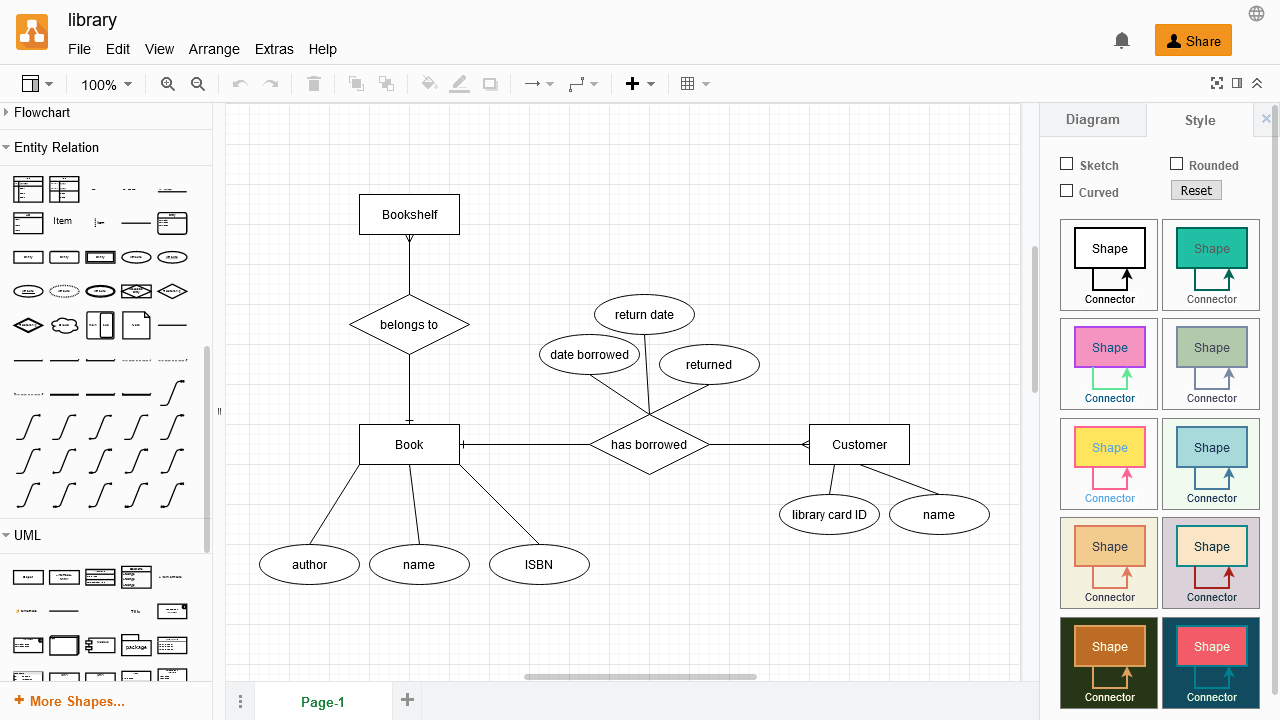
\includegraphics[width = \textwidth]{../img/diagrams.net.png}
  \caption{Tvorba ER diagramu v~aplikaci diagrams.net}
  \label{fig:diagrams.net}
\end{figure}

\section{drawSQL}

Srovnávací kritéria:
\begin{itemize}
  \item kategorie -- logická vrstva,
  \item typ úložiště -- online, poskytované autory produktu
  \item export -- schematický (obecný SQL i~platformě specifické formáty), rastrový \acrshort{png}, serializovaný (JSON~\cite{tc39group_jsondata_2017}, v~době psaní práce se chystá)
  \item interaktivní spolupráce -- pouze v~placené verzi,
  \item komercializace -- omezená verze navždy zdarma, různé měsíčně placené plány.
\end{itemize}

Nástroj drawSQL~\cite{drawsql_2021} je modelovací nástroj pro tvorbu relačních schémat.
Aplikace je dostupná ve webovém prohlížeči\footnote{na adrese \url{https://drawsql.app}}.
Je vyvinuta ve standardních webových technologiích a~používá framework Vue.js.
Plán zdarma umožňuje tvorbu veřejně přístupných diagramů, které mohou mít maximálně 15 tabulek (entit).
Měsíčně placené plány umožňují vytvářet neveřejné diagramy, více (až neomezeně mnoho) tabulek v~diagramu, více uživatelů, kteří mohou na diagramu spolupracovat, a~přístup k~verzovacím nástrojům.
K~vyzkoušení i~používání nástroje je potřeba uživatelský účet.

Hlavní funkcí drawSQL je export schématu do SQL.
Proto si uživatel při vytváření diagramu zvolí cílovou databázi, pro kterou schéma tvoří.
Výsledné SQL tak bude mít tvar, se kterým cílová databáze umí pracovat.
Podporovanými databázemi jsou
MySQL\footnote{\url{https://mysql.com}},
PostgreSQL\footnote{\url{https://postgresql.org}}
a~SQL Server\footnote{Microsoft SQL Server -- \url{https://aka.ms/sqlserver}}.

Rozhraní, které je vidět na Obrázku~\ref{fig:drawsql}, obsahuje diagram a~postranní panel.
V~postranním panelu lze vytvářet jednotlivé tabulky, definovat jejich sloupce a~vlastnosti jednotlivých sloupců -- typ sloupce,
nullability\footnote{\emph{nullability} je příznak, který určuje, zda lze sloupec v~řádku nastavit na hodnotu \texttt{NULL}},
zda se jedná o~primární klíč, unikátní klíč nebo index.
Tyto změny se v~reálném čase reflektují v~diagramu, ve kterém může uživatel jednotlivé sloupce spojovat, čímž vytváří cizí klíče.
Pozici těchto lomených čar lze upravovat pouze posunutím tabulky v~diagramu.
Pokud je cizích klíčů víc, začne být diagram velmi nepřehledný.

Diagram lze importovat ze souboru SQL stisknutím \menu{File > Import}.
Stisknutím tlačítka \menu{File > Export} se otevře nabídka Export, ve které může uživatel diagram exportovat do SQL své předem zvolené databáze, nebo do rastrového obrázku ve formátu \acrshort{png}.
Vývojáři aplikace plánují implementovat také export diagramu pomocí serializace do formátu JSON.
V~nabídce Export je navíc možnost nechat si vygenerovat platformně specifický kód jako například migrační třídy pro
Laravel\footnote{Framework pro PHP -- \url{https://laravel.com}},
definice modelů pro Laravel, a~migrační schémata pro
AdonisJS\footnote{Framework pro Node.js -- \url{https://adonisjs.com}}.

Interaktivní spolupráce je k~dispozici pouze v~placené verzi.
Dle našeho názoru je interaktivní spolupráce hlavní funkcí tohoto nástroje oproti konkurenčním relačním modelovacím nástrojům.
Některá integrovaná vývojová prostředí (např. Visual Studio\footnote{Vývojové prostředí Microsoft Visual Studio -- \url{https://visualstudio.microsoft.com}}) obsahují nástroj pro relační modelování i~generování databázového schématu.
Hlavním omezením těchto nástrojů je však absence interaktivní spolupráce, jedná se spíše o~spolupráci iterací.
Proto považujeme určení interaktivní spolupráce za placenou funkci za negativní rozhodnutí pro využitelnost nástroje v~relaci s~konkurencí.

Web drawSQL také zveřejňuje šablony modelů\footnote{na adrese \url{https://drawsql.app/templates}} (jedná se spíše o~příklady).
Šablony jsou většinou potenciální modely známých produktů (např. WordPress\footnote{\url{https://wordpress.com}}) a~tvoří je autoři drawSQL.
Tuto funkci považujeme za výhodu, protože společnosti a~individuální vývojáři se mohou inspirovat existujícími a~ověřenými řešeními, případně nezačínat se svým modelem od nuly.

Závěrem určíme výhody drawSQL:
\begin{itemize}
  \item příjemné uživatelské rozhraní (viz Obrázek~\ref{fig:drawsql}),
  \item možnost určení typu relace, o~sémantiku se aplikace stará sama (one-to-one, one-to-many, many-to-many),
  \item několik platformě specifických generátorů modelu,
  \item šablony a~příklady existujících modelů
\end{itemize}
a~nevýhody:
\begin{itemize}
  \item nelze upravit ani přesunout lomené čáry spojující cizí klíče, což způsobuje chaos pokud je v~diagramu větší množství entit,
  \item interaktivní spolupráce pouze v~placeném plánu,
  \item správa verzí pouze v~placeném plánu,
  \item k~vyzkoušení nástroje je potřeba uživatelský účet,
  \item podporuje pouze relační databáze.
\end{itemize}

\begin{figure}
  \centering
  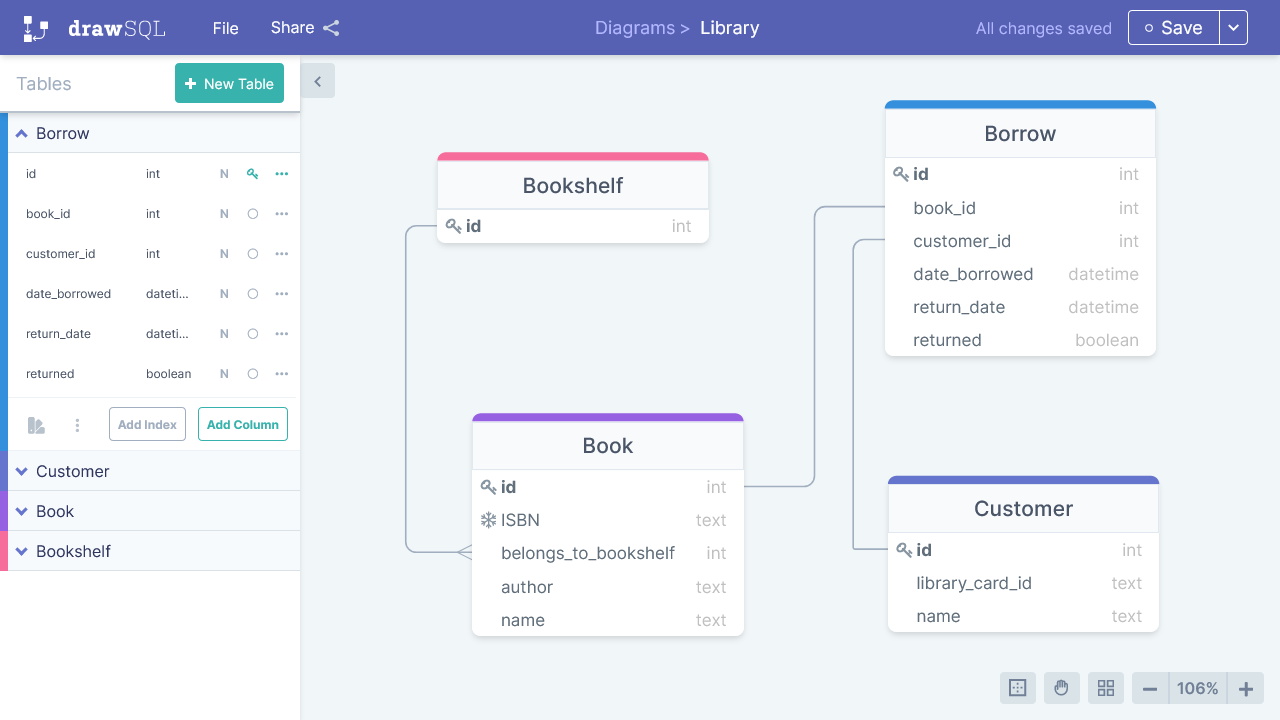
\includegraphics[width = \textwidth]{../img/drawsql.png}
  \caption{Tvorba diagramu v~drawSQL}
  \label{fig:drawsql}
\end{figure}

\section{ERDPlus}
\begin{itemize}
  \item kategorie -- logická vrstva,
  \item typ úložiště -- online, poskytované autory produktu
  \item export -- rastrový \acrshort{png},
  \item interaktivní spolupráce -- není,
  \item komercializace -- zdarma.
\end{itemize}

Nástroj ERDPlus~\cite{erdplus_2023} je modelovací nástroj pro tvorbu ER diagramů, relačních schémat a~hvězdicových schémat.
Aplikace je dostupná ve webovém prohlížeči\footnote{na adrese \url{https://erdplus.com}}.
Její uživatelské rozhraní je tedy vyvinuto ve standardních webových technologiích -- HTML, CSS a~JavaScript.
Dále využívá framework React~\cite{react_2023} pro tvorbu rozhraní v~jazyce JavaScript.

ERDPlus lze používat bez založení uživatelského účtu a~vytvořený diagram exportovat do speciálního formátu erdplus, nicméně uživatel tak přijde o~možnost využití úložiště diagramů na serveru aplikace.
Diagramy (ERDPlus je nazývá \emph{dokumenty}) lze organizovat do složek a podsložek.
Služby ERDPlus včetně úložiště nejsou žádným způsobem zpoplatněny.

Tvorba ER diagramů je intuitivní s~jednoduchým uživatelským rozhraním, které je vidět na Obrázku~\ref{fig:erdplus}.
Uživatel má na výběr mezi vytvořením entity, atributu, relace, spojení mezi těmito objekty a~jednoduchého textového popisku.
V~pravé části rozhraní se nachází panel s~vlastnostmi zvoleného objektu.
V~tomto panelu může uživatel také rychleji tvořit atributy entit a~relací.
Při zvolení relace lze v~panelu zvolit entity, které mají být v~relaci, a~spojení je pak automaticky vytvořeno.
Zároveň lze zvolit jednotlivé multiplicity relace.

Soubor s~diagramem je v~úložišti reprezentován vlastním formátem erdplus.
Jedná se o~textový soubor, jehož obsahem je JSON reprezentace diagramu.
Diagram lze exportovat do rastrového formátu \acrshort{png}.

Zajímavou funkcí je také převod do relačního schématu.
Tato funkce je dostupná pouze tehdy, když uživatel ER diagram uloží na server ERDPlus.
Poté zvolí možnost \emph{Convert to Relational Schema} a~ERDPlus vytvoří nové relační schéma.
Z~relačních schémat lze podobně vygenerovat SQL.

Vlastnoruční tvorba relačních diagramů probíhá podobně.
Uživatel může tvořit tabulky, přidávat jim sloupce a v~tabulkách volit primární klíče v~postranním panelu.
Pomocí tlačítka \texttt{Connect} lze poté přidat cizí klíč, který odkazuje do jiné tabulky tažením myši.
ERDPlus do tabulky přidá všechny primární klíče, které cílová tabulka obsahuje, jako nové sloupce.
K~vytvoření cizího klíče, který odkazuje na stejnou tabulku (tzv. rekurzivní klíč) slouží tlačítko \texttt{Recursive Key} ve vlastnostech tabulky.
Hvězdicovým schématům se věnovat nebudeme, protože jsou mimo rozsah této práce.

Výhody:
\begin{itemize}
  \item převod diagramu z~ER do relačního diagramu,
  \item jednoduchost a intuitivnost procesu kresby diagramu
\end{itemize}
a nevýhody:
\begin{itemize}
  \item relační diagram bývá nepřehledný, nelze měnit pořadí jednotlivých definovaných sloupců v~tabulce,
  \item chybí vektorový export,
  \item diagramy nelze stylizovat.
\end{itemize}

\begin{figure}
  \centering
  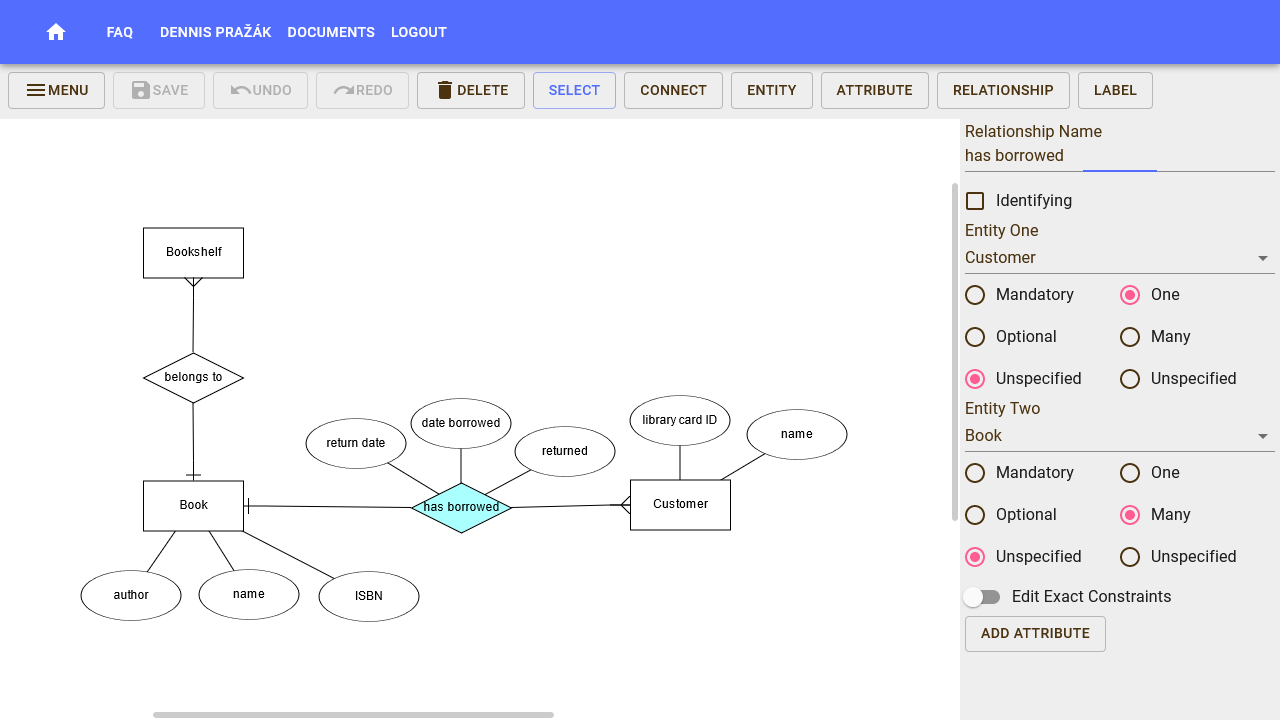
\includegraphics[width = \textwidth]{../img/erdplus.png}
  \caption{Tvorba ER diagramu v~ERDplus}
  \label{fig:erdplus}
\end{figure}

\section{nomnoml}

\begin{itemize}
  \item kategorie -- kresba omezených diagramů -- UML,
  \item typ úložiště -- online,
  \item export -- rastrový \acrshort{png}, vektorový \acrshort{svg},
  \item interaktivní spolupráce -- není k~dispozici,
  \item komercializace -- zdarma s~otevřeným zdrojovým kódem.
\end{itemize}

Nástroj nomnoml je modelovací nástroj pro tvorbu UML diagramů dostupný ve webovém prohlížeči\footnote{na adrese \url{https://nomnoml.com}}.
Jeho klíčová vlastnost je, že místo interakce myší s~webovou aplikací probíhá kresba deklarativně -- psaním.

Uživatelské rozhraní (viz Obrázek~\ref{fig:nomnoml}) se skládá z~oblasti pro textový vstup, nad kterou je zároveň (v~reálném čase) vykreslován výsledný diagram.
V~pravé horní části se nachází několik tlačítek, při kliknutí na některé z~nich se vždy otevře pravý postranní panel s~odpovídajícími informacemi a funkcemi.
První tlačítko ukazuje rychlý přehled jazyka, ve kterém se má diagram definovat.
Druhé tlačítko odhalí kompletní referenci k~tomuto jazyku.
Dále lze najít tlačítka pro export, sdílení a uložení do místního úložiště uživatele.

Jazyk diagramů je velmi jednoduchý.
Skládá se z~definic entit a jejich relací.
Uživatel může vyjít z~úvodního diagramu, který se ukáže při navštívení hlavní stránky nástroje.
Pro ukázku, definice entity vypadá následovně

\noindent\texttt{[<abstract> Entita|soukromaSlozka; soukromaSlozka2|verejnyAtribut]}.

Svislá čára odděluje kategorie atributů, může jich být neomezené množství.
Entita je definována jako abstraktní, což také ovlivní její výsledný styl vzhledu v~diagramu.

Dále se v~jazyce definují vztahy mezi entitami \texttt{[Entita]->[Entita2]}.
Různé šipky mají různé významy.
Vztah \texttt{->} je \emph{asociace}, dále \texttt{o->} je \emph{agregace}, apod.

V~jazyce lze také deklarovat direktivy, začínající znakem \texttt{\#}.
Těmi může uživatel upravit vzhled, vytvořit nové styly, a nastavit algoritmy, kterými bude zvoleno rozložení entit v~diagramu.
Algoritmy lze nastavit direktivou \texttt{\#ranker} a na výběr je ze tří možností: \texttt{network-simplex}, \texttt{tight-tree}, \texttt{longest-path}.
Nástroj nomnoml používá k~vykreslování diagramu knihovnu dagre\footnote{\url{https://github.com/dagrejs/dagre}} pro JavaScript, jejíž vývoj byl však ukončen.
Z~dokumentace této knihovny vyplývá, že možnost \emph{ranker} mění algoritmus, který vrcholům v~grafu (diagramu) přiřazuje důležitost, která se pak odráží v~pořadí zobrazení entit.
Definitivní význam této možnosti není z~dokumentace zřejmý, u~nástroje nomnoml lze však pozorovat změnu v~pořadí a vzdálenostech entit (délce spojovacích čar).
Uživatel tak může vyzkoušet různá rozložení a použít to, které je vizuálně nejpřehlednější.

Diagram lze exportovat do formátu \acrshort{png} a dále podobně jako v~sekci~\ref{section:drawio}, nomnoml také umožňuje export do \acrshort{svg} se zakomponovaným zdrojovým kódem.
Uživatel tak může diagram distribuovat v~tomto formátu a zároveň tento formát v~nástroji nomnoml i otevřít a plnohodnotně pokračovat v~práci.
Podobně je možné sdílet odkaz přímo na vytvořený diagram ve službě nomnoml.
Odkaz je vytvořen tak, že do URL je jako parametr \texttt{source} zapsán přímo zdrojový kód diagramu.
Výsledná adresa URL je tak velice dlouhá, ale služba nomnoml nemusí diagramy ukládat, stačí je vykreslit z~dat v~odkazu.
Přestože se nejedná o~opravdové online úložiště, kategorizovali jsme ho tímto způsobem.
Rozdělaný diagram lze také uložit do paměti prohlížeče.
Díky těmto mechanismům stačí službě nomnoml staticky poskytovat pouze klientskou stranu své aplikace a přesto umožňuje ukládání a sdílení práce.

Nástroj nomnoml je tedy inovativní svým přístupem ke kresbě diagramů.
U~složitých diagramů se však nutně ve zdrojovém kódu uživatel ztrácí, protože nomnoml nenabízí žádné dělení či kompozici tohoto kódu.
S~vizuální reprezentací grafu nelze přímo (např. myší) pracovat, veškeré rozložení a orientaci diagramu tak musí uživatel nechat na algoritmu nástroje.
Nástroj dále nenabízí ani možnost pracovat s~několika diagramy najednou.
Z~těchto důvodů určujeme produkt jako vhodný pouze pro jednotlivce a tvorbu méně rozsáhlých UML diagramů.

\begin{figure}
  \centering
  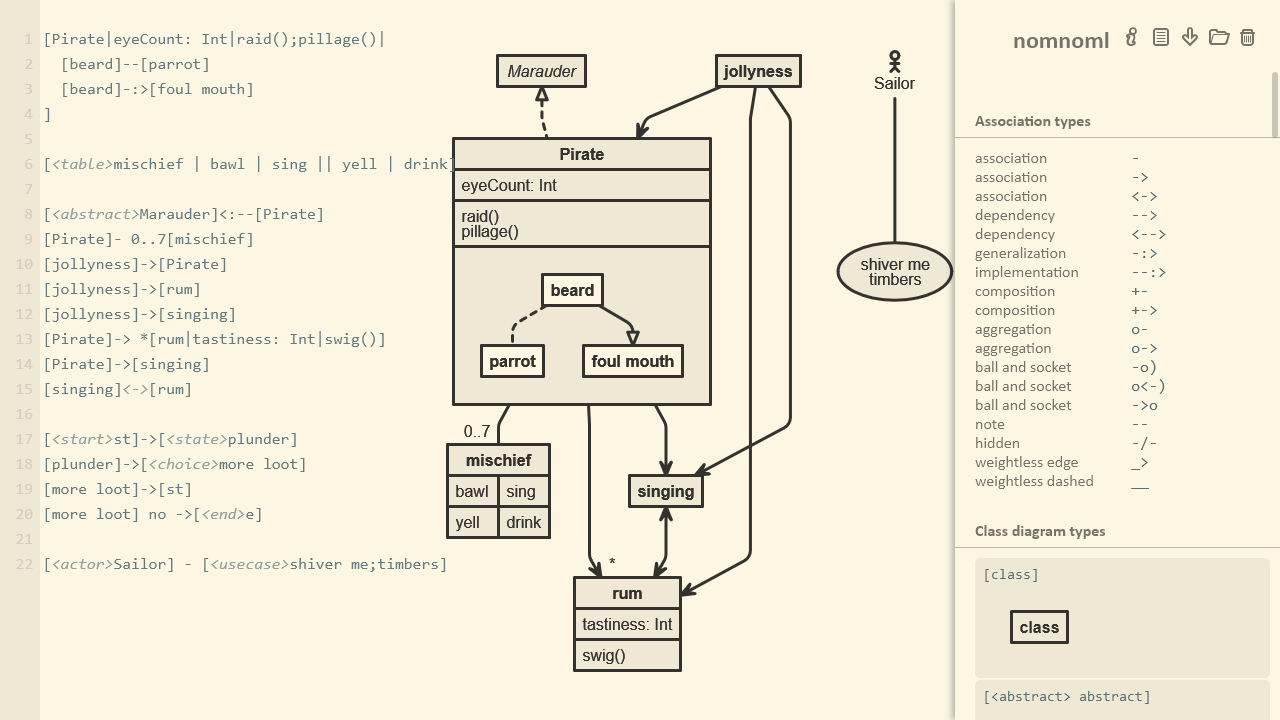
\includegraphics[width = \textwidth]{../img/nomnoml.png}
  \caption{Tvorba UML diagramu v~nomnoml}
  \label{fig:nomnoml}
\end{figure}

\section{Visual Paradigm Online}

Srovnávací kritéria:
\begin{itemize}
  \item kategorie -- kresba libovolných diagramů,
  \item typ úložiště -- online, lokální, externí, prohlížeč,
  \item export -- serializovaný, rastrový, vektorový,
  \item interaktivní spolupráce -- podporována,
  \item komercializace -- verze zdarma, měsíčně/ročně placené plány několika úro\-vní.
\end{itemize}

Nástroj Visual Paradigm Online\footnote{\url{https://online.visual-paradigm.com}} je proprietární produkt od firmy Visual Paradigm.
Tato firma je známá svou stejnojmennou desktopovou aplikací, která má stejný účel. Zde se zaměříme na její online verzi.

Visual Paradigm Online je nástroj pro tvorbu různých typů diagramů.
Mimo těch je určen i pro úpravu fotografií, tvorbu koláží, design infografiky, příspěvků na sociální sítě, uživatelských rozhraní, plakátů, dárkových poukazů, apod.
Funkcionalita kromě tvorby diagramů je mimo rozsah této práce.

Nástroj poskytuje předlohy tvarů pro diagramy tříd, use case diagramy, sekvenční diagramy, diagramy aktivit, diagramy nasazení (deployment), ER diagramy a velmi mnoho dalších.
Uživatel si před tvorbou diagramu musí vybrat jednu z~těchto kategorií, čímž vymezí tvary, které jsou v~uživatelském rozhraní dostupné k~použití v~levém postranním panelu.
Ve stejném panelu lze ale posléze přidat libovolnou další kategorii tvarů dle výběru uživatele.

Nástroj je svým rozhraním, designem a chováním nápadně podobný produktu diagrams.net ze sekce~\ref{section:drawio}.
Stejně tak spojování tvarů čarami má velmi podobné chování.
Jeden rozdíl je ten, že kresba spojení z~jednoho tvaru do toho samého (tvorba "cyklu") je velmi nepředvídatelná.
Čára se při tom samovolně přemisťuje do všech možných stran, až nakonec zůstane přilepena na jedné ze stran tvaru.

Diagramy lze uložit do formátu \texttt{vpd}, který při otevření v~textovém editoru připomíná base64 kód.
Vypadá velice podobně jako serializace pro diagrams.net ze sekce~\ref{section:drawio}.
Nejedná se však o~validní base64 kód, protože ten kóduje 3 bajty do 4 znaků, jinak používá výplň 0-2 znaky \texttt{=}.
Nicméně \texttt{vpd} obsahuje i sekvence jako je \texttt{M=Q8}, které tomu neodpovídají.
Jedná se tak nejspíš o~nezdokumentovaný proprietární formát.

Diagramy lze exportovat do formátu \acrshort{svg} a PDF, do kterých lze volitelně uložit i serializaci diagramu ve formátu \texttt{vpd} a případně tak plnohodnotně přenést editovatelný diagram i s~jeho vektorovou reprezentací.
Rastrový export je možný ve formátu JPEG nebo \acrshort{png}.
Stejně jako u~diagrams.net ze sekce~\ref{section:drawio} je do \acrshort{png} volitelně přidána serializace diagramu v~\texttt{tEXt} chunku formátu \acrshort{png}.
Dokonce je použito stejné klíčové slovo identifikující tuto serializaci -- \texttt{mxfile}.
To vzbuzuje podezření, že se jedná o~stejný formát, jako používá diagrams.net ze sekce \ref{section:drawio}, tedy formát serializace modelu diagramu knihovny mxGraph\footnote{\url{https://jgraph.github.io/mxgraph/}}.
O~tom, že Visual Paradigm Online používá stejný formát jsme ale nenašli žádné zmínky.
Dále, jak už bylo zmíněno, \texttt{vpd} nemá stejnou strukturu jako mxfile\footnote{\url{https://drawio-app.com/extracting-the-xml-from-mxfiles/}}.

Komercializace Visual Paradigm Online je rozdělena do několik platebních úrovní.
Každá úroveň má určenou cenu za uživatele za měsíc.
Úrovně jsou dle ceny a úplnosti funkcí vzestupně Free (zdarma), Starter, Advance, Combo (všechny funkce).
Úroveň Free obsahuje i prémiové šablony, ale je v~nich zobrazen vodoznak.
Ten je v~placených plánech odstraněn.
Placené plány navíc obsahují více typů diagramů a více tvarů k~použití, rastrový export vyššího rozlišení, historii verzí diagramu (při spolupráci) a další.

\section{Závěr existujících řešení}

Přehled analýzy zmíněných existujících řešení je vidět v~Tabulce~\ref{tab:existing-comparison}.

\newcommand{\tnote}[1]{\textsuperscript{#1}}
\begin{table}
  \begin{center}
    \sffamily
    \tabcolsep = 1pt\relax
    \footnotesize
    \makebox[\textwidth]{
      \begin{tabular}{r|c|c|c|c}
        \toprule
        název produktu     & \textbf{diagrams.net}                   & \textbf{drawSQL}                 & \textbf{ERDPlus} & \textbf{nomnoml}                   \\
        \midrule
        kategorie (vrstva) & libovolné d.                            & logická                          & konceptuální     & omezené d.                         \\
        serializovaný ex.  & ano                                     & ne\tnote{\ref{tab:ec:plan}}      & ano              & ano                                \\
        rastrový ex.       & ano                                     & ano                              & ano              & ano                                \\
        vektorový ex.      & ano                                     & ne                               & ne               & ano                                \\
        schematický ex.    & ne                                      & SQL                              & SQL              & ne                                 \\
        zjednodušený ex.   & HTML, PDF                               & ano\tnote{\ref{tab:scaffolding}} & ne               & ne                                 \\
        poskytuje úložiště & ne\tnote{\ref{tab:ec:external-storage}} & ano                              & ano              & ano\tnote{\ref{tab:ec:urlsharing}} \\
        paměť prohlížeče   & ano                                     & ne                               & ne               & ano                                \\
        \midrule[\heavyrulewidth]
      \end{tabular}
    }
  \end{center}

  \footnotesize
  \begin{enumerate}[a.,ref = \alph*,noitemsep]
    \item plánovaná funkce \label{tab:ec:plan}
    \item využívá úložiště třetích stran \label{tab:ec:external-storage}
    \item platformně-specifický scaffolding -- automatické generování kódu pro specifické platformy a programovací jazyky \label{tab:scaffolding}
    \item diagram je uložen v~URL, pomocí které lze diagram sdílet \label{tab:ec:urlsharing}
  \end{enumerate}

  \caption{Srovnání existujících řešení}
  \label{tab:existing-comparison}
\end{table}

\chapter*{Závěr}
\addcontentsline{toc}{chapter}{Závěr}

Závěr

%%% Seznam použité literatury
% %%% Seznam použité literatury (bibliografie)
%%%
%%% Pro vytváření bibliografie používáme bibTeX. Ten zpracovává
%%% citace v textu (např. makro \cite{...}) a vyhledává k nim literaturu
%%% v souboru literatura.bib.
%%%
%%% Příkaz \bibliographystyle určuje, jakým stylem budou citovány odkazy
%%% v textu. V závorce je název zvoleného souboru .bst. Styly plainnat
%%% a unsrt jsou standardní součástí latexových distribucí. Styl czplainnat
%%% je dodáván s touto šablonou a bibTeX ho hledá v aktuálním adresáři.

% \bibliographystyle{czplainnat}    %% Autor (rok) s českými spojkami
% \bibliographystyle{plainnat}    %% Autor (rok) s anglickými spojkami
% \bibliographystyle{unsrt}       %% [číslo], unsorted
\bibliographystyle{unsrturl}       %% [číslo], unsorted + url support

\renewcommand{\bibname}{Seznam použité literatury}

%%% Vytvoření seznamu literatury. Pozor, pokud jste necitovali ani jednu
%%% položku, seznam se automaticky vynechá.

\bibliography{literatura}

%%% Kdybyste chtěli bibliografii vytvářet ručně (bez bibTeXu), lze to udělat
%%% následovně. V takovém případě se řiďte normou ISO 690 a zvyklostmi v oboru.

% \begin{thebibliography}{99}
%
% \bibitem{lamport94}
%   {\sc Lamport,} Leslie.
%   \emph{\LaTeX: A Document Preparation System}.
%   2. vydání.
%   Massachusetts: Addison Wesley, 1994.
%   ISBN 0-201-52983-1.
%
% \end{thebibliography}


%%% Obrázky v bakalářské práci
%%% (pokud jich je malé množství, obvykle není třeba seznam uvádět)
\listoffigures

%%% Tabulky v bakalářské práci (opět nemusí být nutné uvádět)
%%% U matematických prací může být lepší přemístit seznam tabulek na začátek práce.
\listoftables

%%% Použité zkratky v bakalářské práci (opět nemusí být nutné uvádět)
%%% U matematických prací může být lepší přemístit seznam zkratek na začátek práce.

% \chapwithtoc{Seznam použitých zkratek}

%%% Přílohy k bakalářské práci, existují-li. Každá příloha musí být alespoň jednou
%%% odkazována z vlastního textu práce. Přílohy se číslují.
%%%
%%% Do tištěné verze se spíše hodí přílohy, které lze číst a prohlížet (dodatečné
%%% tabulky a grafy, různé textové doplňky, ukázky výstupů z počítačových programů,
%%% apod.). Do elektronické verze se hodí přílohy, které budou spíše používány
%%% v elektronické podobě než čteny (zdrojové kódy programů, datové soubory,
%%% interaktivní grafy apod.). Elektronické přílohy se nahrávají do SISu a lze
%%% je také do práce vložit na CD/DVD. Povolené formáty souborů specifikuje
%%% opatření rektora č. 72/2017.

% \appendix
% \chapter{Přílohy}

% \section{První příloha}

\openright
\end{document}
